%!TEX root = chapter-experiment.tex
\section{Optimizing Parameters}
\label{sec:experiment:parameters}

The database was divided into a training part (the first session of 4000 samples) and a testing part (the second session of 4000 samples). As described in Section ~\ref{ssec:methodology:lda}, the dimension of the proposed  features is $1+N+N\times M$. To select the value of $M$ and $N$, a series of verifications on the training database were carried out where the class of the input palmprint was known. Each of the 3D samples was matched with the remaining samples in the training database. A successful match is where the two samples are from the same class. This is referred to as intra-class matching and the candidate image is said to be genuine. An unsuccessful match is referred to as inter-class matching and the candidate image is said to be an impostor. Treating the features as a point in the $1+N+N\times M$ dimension space, Euclidian distance is used as the matching score.


%!TEX root = chapter-experiment.tex
\section{Optimizing Parameters}
\label{sec:experiment:parameters}

The database was divided into a training part (the first session of 4000 samples) and a testing part (the second session of 4000 samples). As described in Section ~\ref{ssec:methodology:lda}, the dimension of the proposed  features is $1+N+N\times M$. To select the value of $M$ and $N$, a series of verifications on the training database were carried out where the class of the input palmprint was known. Each of the 3D samples was matched with the remaining samples in the training database. A successful match is where the two samples are from the same class. This is referred to as intra-class matching and the candidate image is said to be genuine. An unsuccessful match is referred to as inter-class matching and the candidate image is said to be an impostor. Treating the features as a point in the $1+N+N\times M$ dimension space, Euclidian distance is used as the matching score.


%!TEX root = chapter-experiment.tex
\section{Optimizing Parameters}
\label{sec:experiment:parameters}

The database was divided into a training part (the first session of 4000 samples) and a testing part (the second session of 4000 samples). As described in Section ~\ref{ssec:methodology:lda}, the dimension of the proposed  features is $1+N+N\times M$. To select the value of $M$ and $N$, a series of verifications on the training database were carried out where the class of the input palmprint was known. Each of the 3D samples was matched with the remaining samples in the training database. A successful match is where the two samples are from the same class. This is referred to as intra-class matching and the candidate image is said to be genuine. An unsuccessful match is referred to as inter-class matching and the candidate image is said to be an impostor. Treating the features as a point in the $1+N+N\times M$ dimension space, Euclidian distance is used as the matching score.


%!TEX root = chapter-experiment.tex
\section{Optimizing Parameters}
\label{sec:experiment:parameters}

The database was divided into a training part (the first session of 4000 samples) and a testing part (the second session of 4000 samples). As described in Section ~\ref{ssec:methodology:lda}, the dimension of the proposed  features is $1+N+N\times M$. To select the value of $M$ and $N$, a series of verifications on the training database were carried out where the class of the input palmprint was known. Each of the 3D samples was matched with the remaining samples in the training database. A successful match is where the two samples are from the same class. This is referred to as intra-class matching and the candidate image is said to be genuine. An unsuccessful match is referred to as inter-class matching and the candidate image is said to be an impostor. Treating the features as a point in the $1+N+N\times M$ dimension space, Euclidian distance is used as the matching score.


\input{ch-experiment/tables/parameters}

Table ~\ref{tab:experiment:parameters} shows the Equal Error Rate (EER) for $N=4,8,16$ and $M=8,16,32,64$. The best result, as adopted in Chapter ~\ref{ch:methodology}, is $N=8$ and $M=32$.


In order to balance accuracy and efficiency, we chose $N=8$ and $M=32$ in the following experiments. This means the features have $1+N+N\times M=265$ dimensions.

\input{ch-experiment/tables/verification}

Table ~\ref{tab:experiment:verification} shows the verification results by MD, HCA, RLL and their combined results. From the last column of Table ~\ref{tab:experiment:verification} we can see using the combined three features will achieve a lower EER than each of the individual features.

As described in Section ~\ref{ssec:methodology:lda}, we use the OLDA method to reduce features to a lower dimension $\Gamma$. To decide the optimal value of $\Gamma$, we carried out a series of recognition experiments on the 4000 sample training database. We divided this database into two equal parts and then chose the first five samples of every palm for training and set aside the rest for testing. As shown in Section ~\ref{ssec:methodology:lda}, $\Gamma$ is equal to q in (13). Instead of setting $q=rank(B)$, we set $q=1,2,\dots,10,12,15,20,30$.

\input{ch-experiment/tables/gamma}

Table ~\ref{tab:experiment:gamma} shows the recognition results.

\begin{figure}[htb]
  \begin{center}
    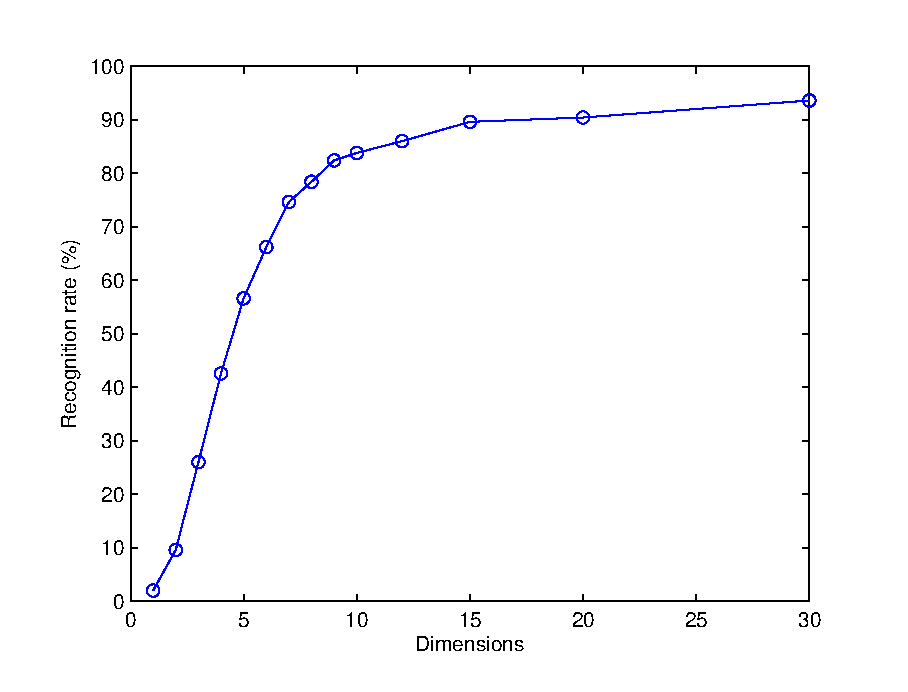
\includegraphics[width=\linewidth]{ch-experiment/figures/gamma}
    \caption[Recognition rate by OLDA for different dimensions]{Recognition rate by OLDA for different dimensions}
    \label{fig:experiment:gamma}
  \end{center}
\end{figure}

According to the curve shown in Figure ~\ref{fig:experiment:gamma}, $\Gamma=15$ is a good choice for the following experiments with balanced recognition rate and computation.

Table ~\ref{tab:experiment:parameters} shows the Equal Error Rate (EER) for $N=4,8,16$ and $M=8,16,32,64$. The best result, as adopted in Chapter ~\ref{ch:methodology}, is $N=8$ and $M=32$.


In order to balance accuracy and efficiency, we chose $N=8$ and $M=32$ in the following experiments. This means the features have $1+N+N\times M=265$ dimensions.

% Table generated by Excel2LaTeX from sheet 'Sheet2'
\begin{table}[htbp]
  \centering
  \caption{The EER of 3D palmprint verification for with each feature and the combined feature}
    \begin{tabular}{ccccc}
    \toprule
    Global features & MD    & HCA   & RLL   & MD+HCA+RLL \\
    \midrule
    EER(\%) & 25.8  & 20.4  & 18.6  & 12.32 \\
    \bottomrule
    \end{tabular}%
  \label{tab:experiment:verification}%
\end{table}%


Table ~\ref{tab:experiment:verification} shows the verification results by MD, HCA, RLL and their combined results. From the last column of Table ~\ref{tab:experiment:verification} we can see using the combined three features will achieve a lower EER than each of the individual features.

As described in Section ~\ref{ssec:methodology:lda}, we use the OLDA method to reduce features to a lower dimension $\Gamma$. To decide the optimal value of $\Gamma$, we carried out a series of recognition experiments on the 4000 sample training database. We divided this database into two equal parts and then chose the first five samples of every palm for training and set aside the rest for testing. As shown in Section ~\ref{ssec:methodology:lda}, $\Gamma$ is equal to q in (13). Instead of setting $q=rank(B)$, we set $q=1,2,\dots,10,12,15,20,30$.

% Table generated by Excel2LaTeX from sheet 'Sheet3'
\begin{table}[htbp]
  \centering
  \caption{Recognition rate by OLDA for different dimensions}
    \tabcolsep=0.11cm
    \begin{tabular}{|r|c|c|c|c|c|c|c|c|c|c|c|c|c|c|}
    \hline
        $\Gamma$  & 1     & 2     & 3     & 4     & 5     & 6     & 7     & 8     & 9     & 10    & 12    & 15    & 20    & 30 \\
    \hline
    Recognition rate (\%) & {2} & {9.6} & {26} & {42.6} & {56.6} & {66.2} & {74.6} & {78.4} & {82.4} & {83.8} & {86} & {89.6} & {90.4} & {93.6} \\
	\hline
    \end{tabular}%
  \label{tab:experiment:gamma}%
\end{table}%


Table ~\ref{tab:experiment:gamma} shows the recognition results.

\begin{figure}[htb]
  \begin{center}
    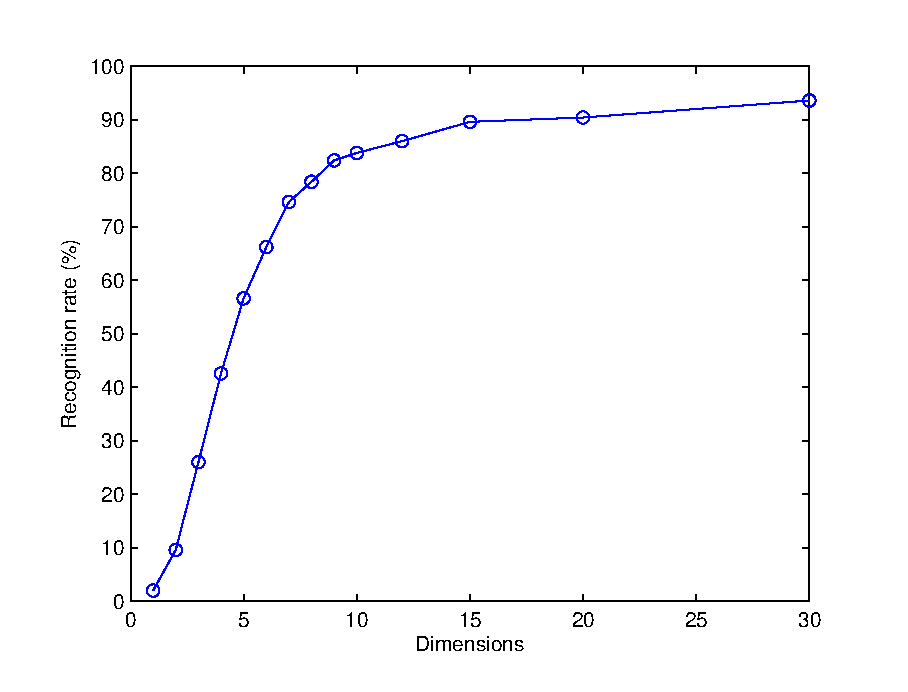
\includegraphics[width=\linewidth]{ch-experiment/figures/gamma}
    \caption[Recognition rate by OLDA for different dimensions]{Recognition rate by OLDA for different dimensions}
    \label{fig:experiment:gamma}
  \end{center}
\end{figure}

According to the curve shown in Figure ~\ref{fig:experiment:gamma}, $\Gamma=15$ is a good choice for the following experiments with balanced recognition rate and computation.

Table ~\ref{tab:experiment:parameters} shows the Equal Error Rate (EER) for $N=4,8,16$ and $M=8,16,32,64$. The best result, as adopted in Chapter ~\ref{ch:methodology}, is $N=8$ and $M=32$.


In order to balance accuracy and efficiency, we chose $N=8$ and $M=32$ in the following experiments. This means the features have $1+N+N\times M=265$ dimensions.

% Table generated by Excel2LaTeX from sheet 'Sheet2'
\begin{table}[htbp]
  \centering
  \caption{The EER of 3D palmprint verification for with each feature and the combined feature}
    \begin{tabular}{ccccc}
    \toprule
    Global features & MD    & HCA   & RLL   & MD+HCA+RLL \\
    \midrule
    EER(\%) & 25.8  & 20.4  & 18.6  & 12.32 \\
    \bottomrule
    \end{tabular}%
  \label{tab:experiment:verification}%
\end{table}%


Table ~\ref{tab:experiment:verification} shows the verification results by MD, HCA, RLL and their combined results. From the last column of Table ~\ref{tab:experiment:verification} we can see using the combined three features will achieve a lower EER than each of the individual features.

As described in Section ~\ref{ssec:methodology:lda}, we use the OLDA method to reduce features to a lower dimension $\Gamma$. To decide the optimal value of $\Gamma$, we carried out a series of recognition experiments on the 4000 sample training database. We divided this database into two equal parts and then chose the first five samples of every palm for training and set aside the rest for testing. As shown in Section ~\ref{ssec:methodology:lda}, $\Gamma$ is equal to q in (13). Instead of setting $q=rank(B)$, we set $q=1,2,\dots,10,12,15,20,30$.

% Table generated by Excel2LaTeX from sheet 'Sheet3'
\begin{table}[htbp]
  \centering
  \caption{Recognition rate by OLDA for different dimensions}
    \tabcolsep=0.11cm
    \begin{tabular}{|r|c|c|c|c|c|c|c|c|c|c|c|c|c|c|}
    \hline
        $\Gamma$  & 1     & 2     & 3     & 4     & 5     & 6     & 7     & 8     & 9     & 10    & 12    & 15    & 20    & 30 \\
    \hline
    Recognition rate (\%) & {2} & {9.6} & {26} & {42.6} & {56.6} & {66.2} & {74.6} & {78.4} & {82.4} & {83.8} & {86} & {89.6} & {90.4} & {93.6} \\
	\hline
    \end{tabular}%
  \label{tab:experiment:gamma}%
\end{table}%


Table ~\ref{tab:experiment:gamma} shows the recognition results.

\begin{figure}[htb]
  \begin{center}
    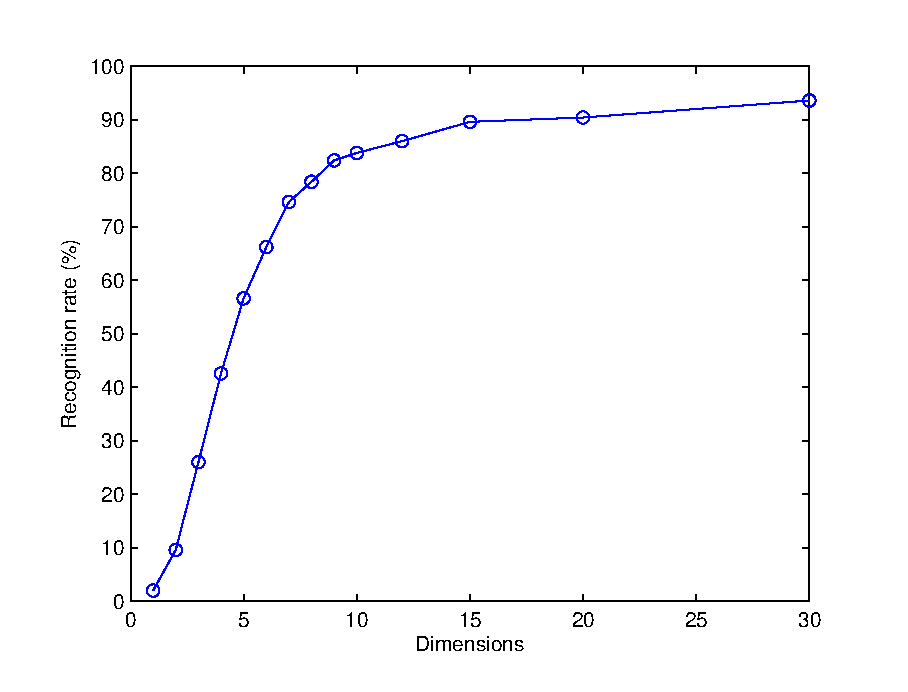
\includegraphics[width=\linewidth]{ch-experiment/figures/gamma}
    \caption[Recognition rate by OLDA for different dimensions]{Recognition rate by OLDA for different dimensions}
    \label{fig:experiment:gamma}
  \end{center}
\end{figure}

According to the curve shown in Figure ~\ref{fig:experiment:gamma}, $\Gamma=15$ is a good choice for the following experiments with balanced recognition rate and computation.

Table ~\ref{tab:experiment:parameters} shows the Equal Error Rate (EER) for $N=4,8,16$ and $M=8,16,32,64$. The best result, as adopted in Chapter ~\ref{ch:methodology}, is $N=8$ and $M=32$.


In order to balance accuracy and efficiency, we chose $N=8$ and $M=32$ in the following experiments. This means the features have $1+N+N\times M=265$ dimensions.

% Table generated by Excel2LaTeX from sheet 'Sheet2'
\begin{table}[htbp]
  \centering
  \caption{The EER of 3D palmprint verification for with each feature and the combined feature}
    \begin{tabular}{ccccc}
    \toprule
    Global features & MD    & HCA   & RLL   & MD+HCA+RLL \\
    \midrule
    EER(\%) & 25.8  & 20.4  & 18.6  & 12.32 \\
    \bottomrule
    \end{tabular}%
  \label{tab:experiment:verification}%
\end{table}%


Table ~\ref{tab:experiment:verification} shows the verification results by MD, HCA, RLL and their combined results. From the last column of Table ~\ref{tab:experiment:verification} we can see using the combined three features will achieve a lower EER than each of the individual features.

As described in Section ~\ref{ssec:methodology:lda}, we use the OLDA method to reduce features to a lower dimension $\Gamma$. To decide the optimal value of $\Gamma$, we carried out a series of recognition experiments on the 4000 sample training database. We divided this database into two equal parts and then chose the first five samples of every palm for training and set aside the rest for testing. As shown in Section ~\ref{ssec:methodology:lda}, $\Gamma$ is equal to q in (13). Instead of setting $q=rank(B)$, we set $q=1,2,\dots,10,12,15,20,30$.

% Table generated by Excel2LaTeX from sheet 'Sheet3'
\begin{table}[htbp]
  \centering
  \caption{Recognition rate by OLDA for different dimensions}
    \tabcolsep=0.11cm
    \begin{tabular}{|r|c|c|c|c|c|c|c|c|c|c|c|c|c|c|}
    \hline
        $\Gamma$  & 1     & 2     & 3     & 4     & 5     & 6     & 7     & 8     & 9     & 10    & 12    & 15    & 20    & 30 \\
    \hline
    Recognition rate (\%) & {2} & {9.6} & {26} & {42.6} & {56.6} & {66.2} & {74.6} & {78.4} & {82.4} & {83.8} & {86} & {89.6} & {90.4} & {93.6} \\
	\hline
    \end{tabular}%
  \label{tab:experiment:gamma}%
\end{table}%


Table ~\ref{tab:experiment:gamma} shows the recognition results.

\begin{figure}[htb]
\begin{center}
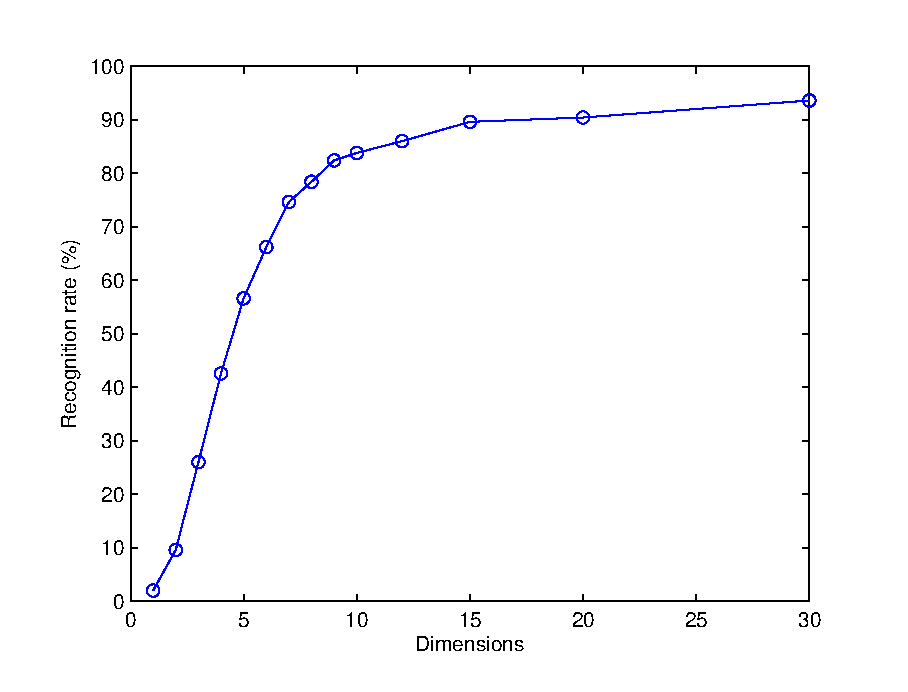
\includegraphics[width=\linewidth]{ch-experiment/figures/gamma}
\caption[Recognition rate by OLDA for different dimensions]{Recognition rate by OLDA for different dimensions}
\label{fig:experiment:gamma}
\end{center}
\end{figure}

According to the curve shown in Figure ~\ref{fig:experiment:gamma}, $\Gamma=15$ is a good choice for the following experiments with balanced recognition rate and computation.